\section{Process Architecture}
In this section two distribution diagrams will be shown which explains the processor, the active objects and their connections. All the systems components is on a single processor, but there is going to be multiple processors which is communication with the database. This is due to the system being designed to run on a single device that is not dependent on other devices.

\subsection{Distribution diagrams}
The first distribution diagram will be for the Shopping List.

\begin{figure}[H]
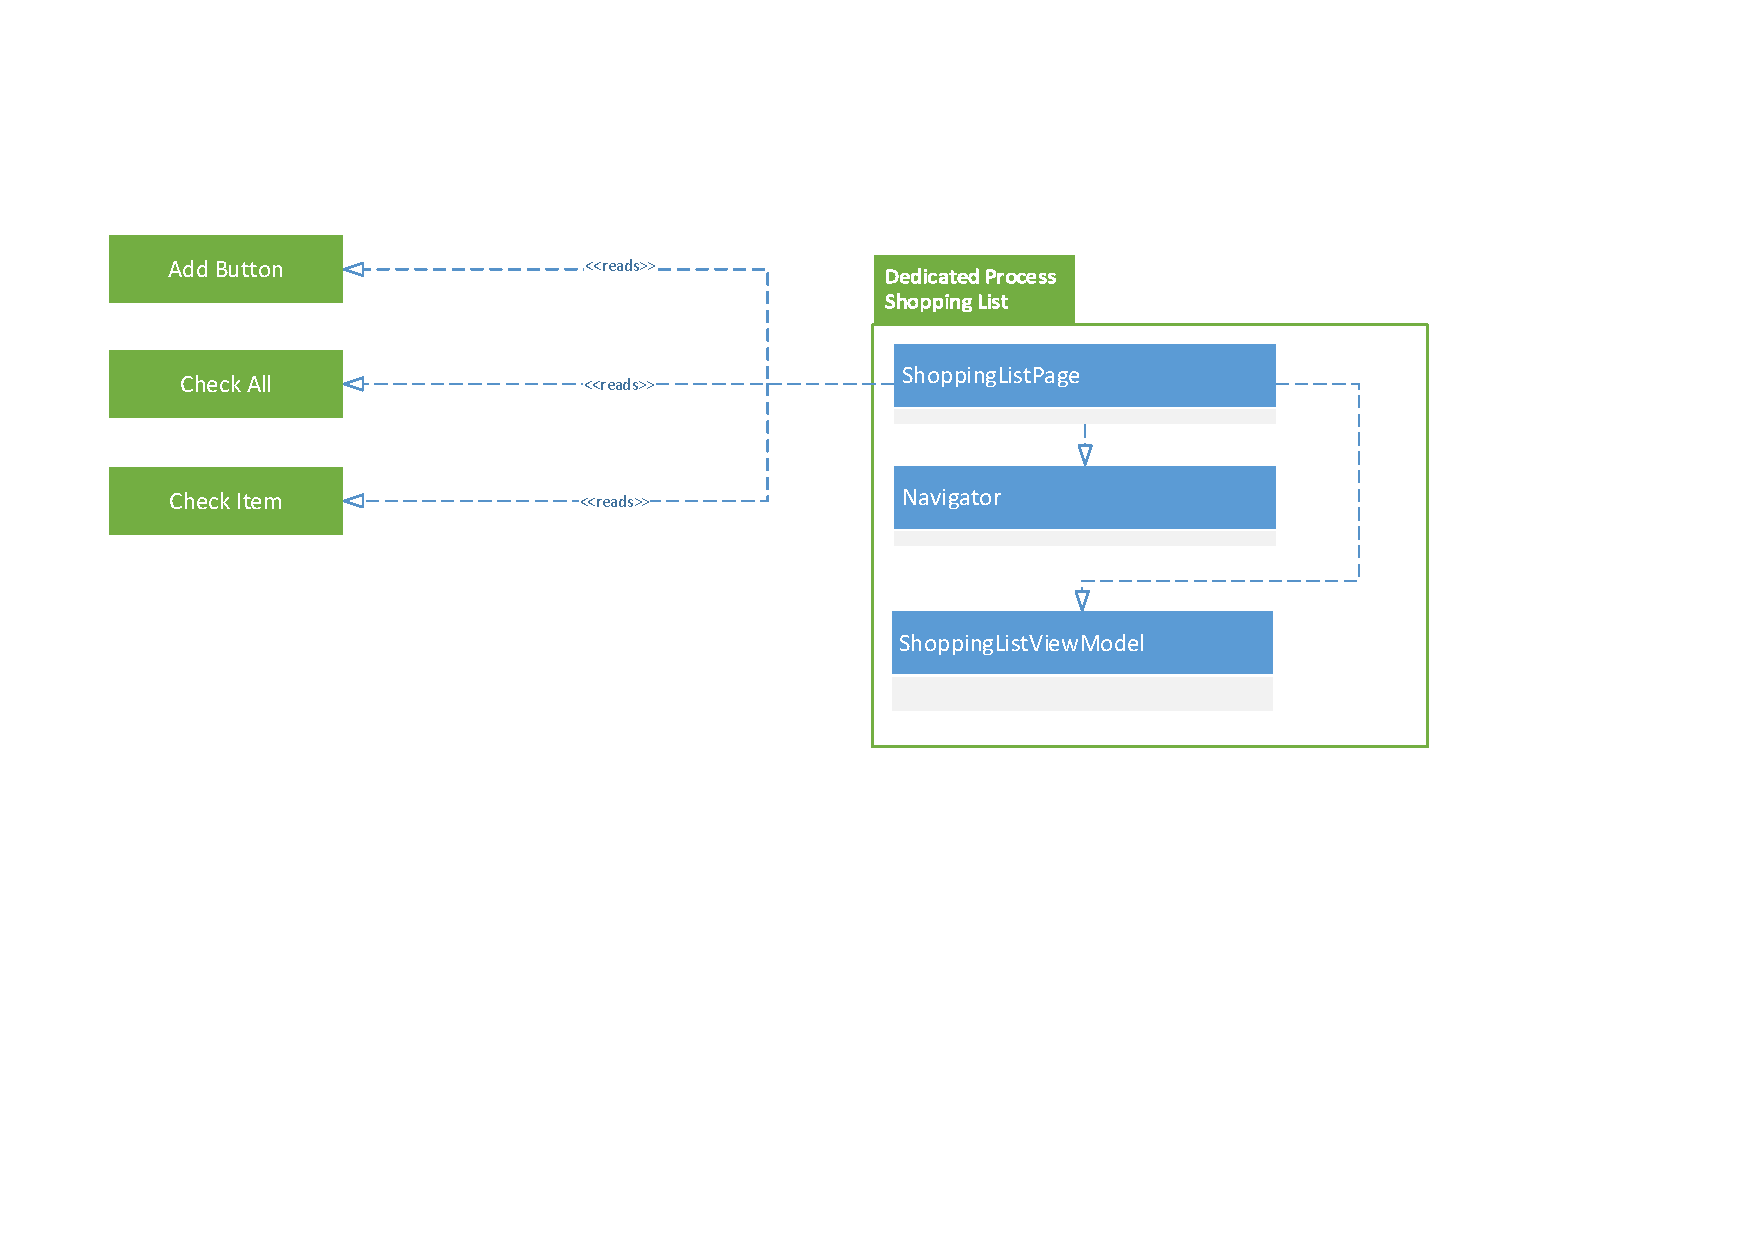
\includegraphics[width=\linewidth]{Grafik/FoodPlanner/DistributionShoppingList}
\centering
\caption{The distribution diagram for the Shopping List}
\label{SLD}
\end{figure}

\Cref{SLD} shows three active objects:
\begin{itemize}
\item Add Button 
- This object adds the checked items on the shopping list to the inventory
\item Check All 
- Checks all items on the shopping list 
\item Check Item 
- Checks an single item on the shopping list
\end{itemize}

\begin{figure}[H]
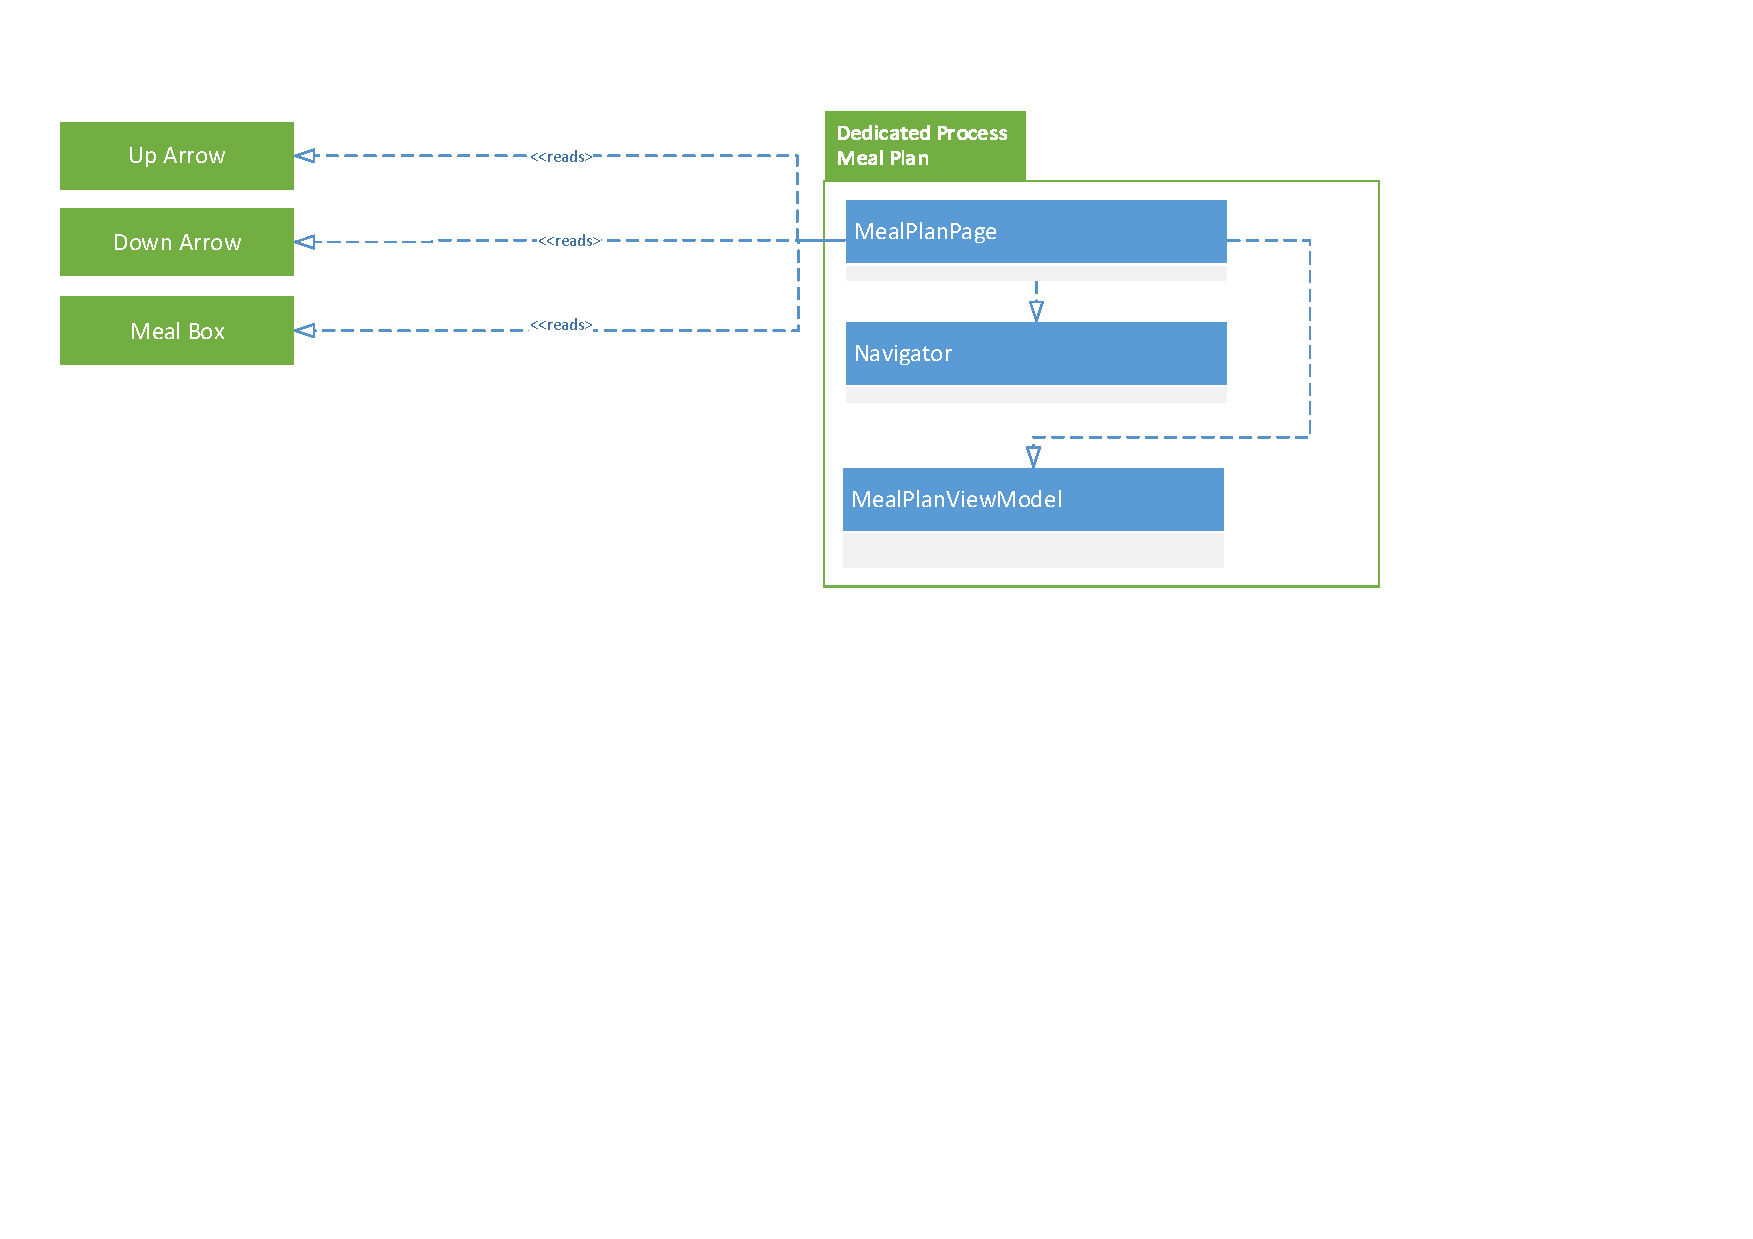
\includegraphics[width=\linewidth]{Grafik/FoodPlanner/DistributionMealPlan}
\centering
\caption{The distribution diagram for the Meal Plan}
\label{MPD}
\end{figure}

\Cref{MPD} shows three active objects:
\begin{itemize}
\item Up Arrow 
- Displays the previous week
\item Down Arrow 
- Shows the next week
\item Meal Box 
- Sends the user to the Recipe Page
\end{itemize}

The next diagram shows the distribution pattern that have been used.

\begin{figure}[H]
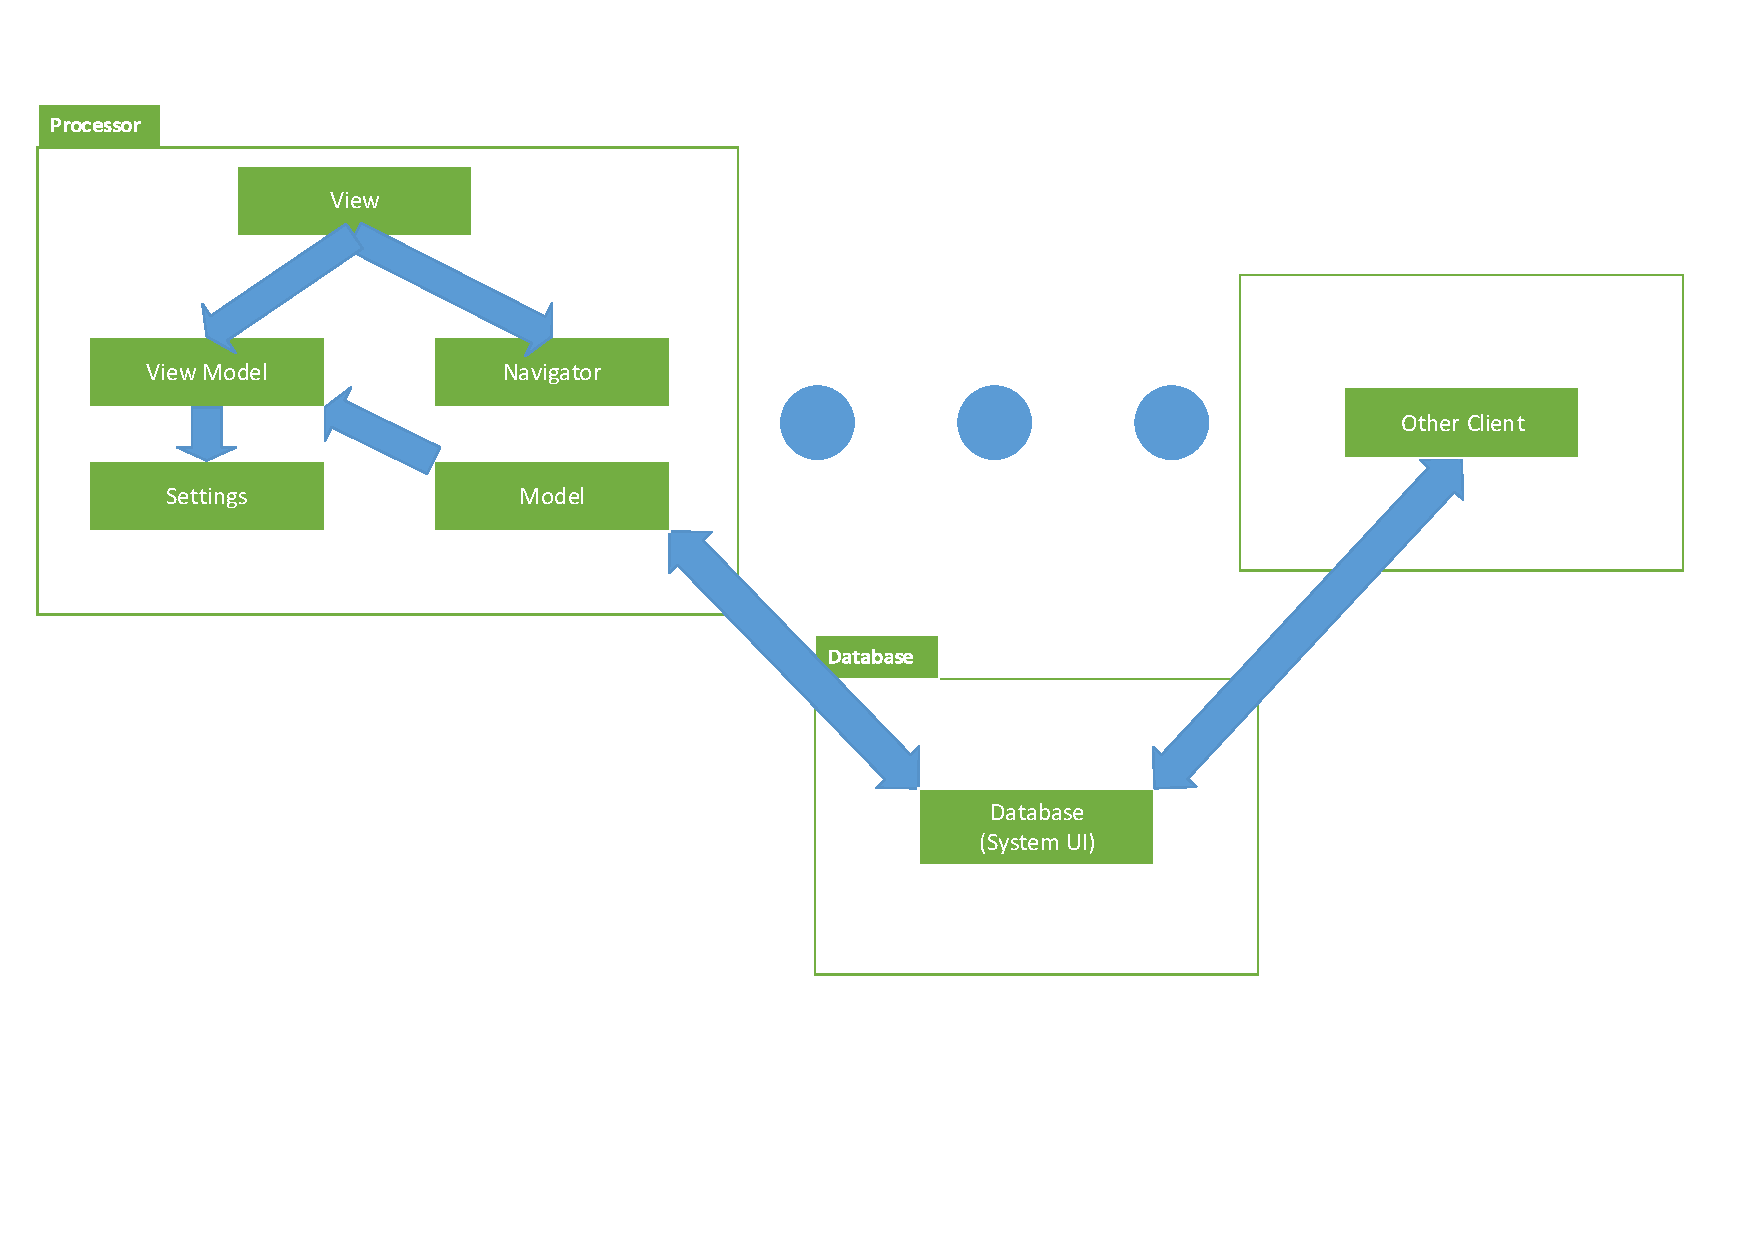
\includegraphics[width=\linewidth]{Grafik/FoodPlanner/FordelingsDiagram}
\centering
\caption{The used distribution pattern}
\label{DP}
\end{figure}

\Cref{DP} shows the distribution pattern that have been used, which is a similar pattern to the centralized pattern. Normally the server will perform the functions and keep the model on itself whereas in this system, the client will perform all the functions and still have some local data which is the settings. A downside to this model lies in the stability, as the system is only functional when a clear connection to the server is established. Another downside to the model is the connection time as almost every interaction with the system will require it to communicate with the server. The server communication creates a natural bottleneck in the system as a server can only handle so much data at any time. When the user searches for a recipe, the entire list of recipes will be looked through in order to acquire the matching results. If it were possible to cash data such as recipes or ingredients, data that does not change often, it would loosen up the bottleneck.